\begin{marginfigure}[2cm] % MARGIN FIGURE
\begin{center}
\subfloat[$f_1(x) = 1/x^2$]{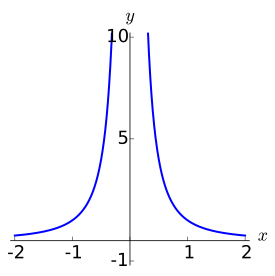
\includegraphics[scale=.3]{figs/3/activity351a.pdf}}
\hspace{.25cm}
\subfloat[$f_2(x) = |x|$]{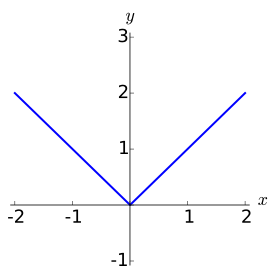
\includegraphics[scale=.3]{figs/3/activity351b.pdf}}
\caption{The functions $f_1(x) = 1/x^2$ and $f_2(x) = |x|$ used in Activity~\ref{A:3.5.1}}
\label{fig:act351}
\end{center}
\end{marginfigure}

\begin{activity} \label{A:3.5.1}  Consider functions 
$$f_1(x)=\frac{1}{x^2}\quad \text{and} \quad f_2(x) = |x|$$ 
with $a=-1$ and $b=1$ as shown in Figure~\ref{fig:act351}-(a) and -(b), respectively. 
\ba
 \item For $f_1(x)$, find the slope of the secant line connecting the points $(a,f(a))$ and $(b,f(b))$.
 \item Find a value $c$ in $(a,b)$ such that $f_1'(c)$ equals the slope of the secant line connecting the points $(a,f(a))$ and $(b,f(b))$. Was it possible to find $c$? If not, what went wrong?
  \item For $f_2(x)$, find the slope of the secant line connecting the points $(a,f(a))$ and $(b,f(b))$.
 \item Find a value $c$ in $(a,b)$ such that $f_2'(c)$ equals the slope of the secant line connecting the points $(a,f(a))$ and $(b,f(b))$. Was it possible to find $c$? If not, what went wrong?
	\ea
\end{activity}

\aftera